% arara: lualatex: { synctex: yes, shell: yes } 
% arara: biber 
% arara: lualatex if changed("bib")
% if changed("bib")

% % -*- coding:utf-8 -*-
\documentclass[aspectratio=169,10pt, notes]{beamer}
\nonstopmode

% Basic Packages
%\usepackage[utf8]{inputenc}
%\usepackage[T1]{fontenc}
\usepackage[ngerman]{babel}

% Geometry
\usepackage[a4paper,
            bindingoffset=0.2in,
            left=1.5in,
            right=1.5in,
            top=1in,
            bottom=1in,
            footskip=.3in]{geometry}
            
% Textstuff
\usepackage{csquotes}
\usepackage{url}
\usepackage{hyperref}
\usepackage{lmodern}            % Provides the Latin Modern Font which offers more glyphs than the default Computer Modern
\usepackage[nameinlink]{cleveref}
\crefname{figure}{Abbildung}{Abbildung}
\crefname{subfigure}{Abbildung}{Abbildung}
\crefname{table}{Tabelle}{Tabelle}
\crefname{listing}{Quelltext}{Quelltext}
\crefname{chapter}{Kapitel}{Kapitel}
\crefname{section}{Abschnitt}{Abschnitt}
\crefname{subsection}{Abschnitt}{Abschnitt}
\crefname{subsubsection}{Abschnitt}{Abschnitt}
\crefname{beispiel}{Beispiel}{Beispiel}
\crefname{lemma}{Lemma}{Lemma}

% Set Paragraph Skip
\setlength{\parskip}{0.5\baselineskip}%
\setlength{\parindent}{0pt}%

% gfx
\usepackage{pgfpages}
\usepackage{svg}
\usepackage{graphicx}
\usepackage{xcolor}
\usepackage{color}
\usepackage{wrapfig}

% Tikz
\usepackage{tikz}
\usetikzlibrary{positioning,calc}

% Bibliography
\usepackage{biblatex}
\addbibresource{ethik.bib}




\title{Faites Vos Jeux}
\subtitle{So viele Daten sind das ja nicht... oder?}
\author{Etienne Palanga}
\date{2. Juni 2022}
\institute{TU Dortmund - Fakultät Informatik}
\titlegraphic{\hfill
\includegraphics[height=8mm]{tu-do-logo.pdf}}

\begin{document}

\maketitle

\begin{frame}{Inhaltsverzeichnis}
    \tableofcontents
\end{frame}


\section{Einleitung}

\begin{frame}{Datenschutz}
  \centering 
  
  \note[item]{Überall werden Daten erhoben}
  \note[item]{
    Manchmal eindeutig 
    \begin{itemize}
      \item Eingabe von Daten bei Kontoerstellung
    \end{itemize}
  }
  \note[item]{
    Aber viel öfter ohne wirkliches Wissen
    \begin{itemize}
      \item Tracker auf Websites
      \item Nutzung anderer Dienste
    \end{itemize}
  }
  \note[item]{
    Deswegen Datenschutz wichtig
  }

  
\includegraphics[width=0.45\textwidth]{images/computer_data_tobu} 
\end{frame}

\begin{frame}{Datenschutz}

  \note<1->[item]{Definition aus Paper von Lee et al. (meine Zusammenfassung u. Übersetzung)}
  \note<2->[item]{Schutz vor unauthorisiertem Zugriff}
  \note<3->[item]{Sicherung, dass die Daten angemessen genutzt werden}
  \note<4->[item]{Korrektheit und Vollständigkeit gesammelter Daten über Personen}
  \note<5->[item]{Verfügbarkeit der Daten für das Subjekt und die Sicherung der Rechte des Subjekts an seinen Daten}
  \note<6->[item]{Sicherung der Rechte des Subjekts die Daten einzusehen, aktualisieren oder korrigieren}

  Nach Lee et al.\cite{lee_ethical_2016}:

  \begin{block}{Datenschutz}
    \begin{itemize}
      \item<2->{Schutz vor unauthorisiertem Zugriff}
      \item<3->{Sicherung, dass die Daten angemessen genutzt werden}
      \item<4->{Korrektheit und Vollständigkeit gesammelter Daten über Personen}
      \item<5->{Verfügbarkeit der Daten für das Subjekt und das Besitzrecht des Subjekts an seinen Daten}
      \item<6->{Sicherung der Rechte des Subjekts die Daten einzusehen, aktualisieren oder korrigieren}
    \end{itemize} 
  \end{block}
\end{frame}

\begin{frame}{Datenschutz}
  \centering

  \note<1->[item]{Selbes Paper}
  \note<1->[item]{Gesetz und Ethik sind verbunden}
  \note<2->[item]{Gesetz gibt Ethik Durchsetzungsvermögen \begin{itemize}
      \item Bsp. Ethischer Schluss: Stehlen ist falsch
      \item Aber ohne Gesetz: keine Durchsetzung
    \end{itemize}
  }
  \note<3->[item]{Ethik gibt Gesetz Kontext \begin{itemize}
      \item Bsp. Arbeit in Niedriglohnländer auszulagern ist legal, aber ist es ethisch?
    \end{itemize}
  }
  \note<3->[item]{Ethische Ideen über Datenschutz werden im Gesetz umgesetzt.}
  \note<3->[item]{Sehen das später etwas mehr}

  \begin{tikzpicture}
    \node (law) {
\includegraphics[width=0.25\textwidth]{images/book_law}};
    \node[below = 0cm of law] (law-name) {Gesetz};
    \node[right = 4cm of law] (ethics) {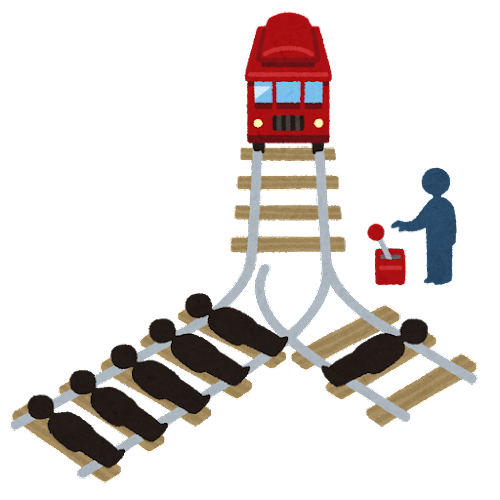
\includegraphics[width=0.25\textwidth]{images/trolley_problem}};
    \node[below = 0cm of ethics] (ethics-name) {Ethik};

    \draw<2->[-stealth] (law) to[out = 20, in = 160, edge node={node[above] {Kann durchsetzen}}] (ethics);
    \draw<3->[-stealth] (ethics) to[out = 200, in = 340, edge node={node[below] {Gibt Kontext}}] (law);
  \end{tikzpicture}

\end{frame}



\section{Faites Vos Jeux \cite{kees_faites_2017}}

\note{\begin{itemize}
    \item Fallbeispiel aus Informatik Spektrum 2017
\end{itemize}}

\begin{frame}{Anfänge von AC-Games}
  \centering
  
  \note[item]<1->{
    Walter \begin{itemize}
      \item Unternehmer seit fast 2 Jahrzehnten
    \end{itemize}
  }
  \note[item]<2->{
    Geschäftsführer Firma AC-Games \begin{itemize}
      \item Betreibt kostenlose Spieleportal für Online-Spiele im Internet
    \end{itemize} 
  }
  \note[item]<3->{ Relativ großer Kundenstamm \begin{itemize}
      \item Finanzierung mit nur 100 aktivsten Spielern \begin{itemize}
        \item Werbung
        \item Kauf virtueller Gegenstände
      \end{itemize}
      \item Firma läuft gut
      \item Aber wären ja nicht hier wenn nicht irgendwas schief geht
    \end{itemize}
  }
  
  \begin{tikzpicture}
    \node<1-> (walter) {
\includegraphics[width=0.15\textwidth]{images/walter.png}};
    \node<1->[below=0mm of walter] (walter-name) {Walter};
    
    
    \node<2->[left=3cm of walter] (acgames) {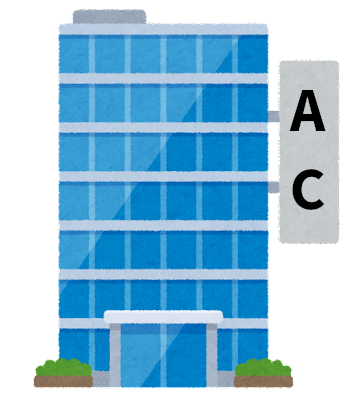
\includegraphics[width=0.15\textwidth]{images/ac_games.png}};
    \node<2->[below=0cm of acgames] (acgames-name) {AC-Games};
    
    \node<3->[left=3cm of acgames] (nutzer) {
\includegraphics[width=0.15\textwidth]{images/game_friends.png}};
    \node<3->[below=0cm of nutzer] (nutzer-name) {Nutzer:innen};
    
    \draw<2->[-stealth] (walter) -- node[below] {CEO}  (acgames);
    \draw<3->[-stealth] (nutzer) -- node[below] (geld) {Geld} (acgames);
  \end{tikzpicture} 
\end{frame}

\begin{frame}{Finanzkrise}
  \centering
  
  \note[item]<1-> {Gibt jetzt Probleme}
  \note[item]<2-> {Finanzkrise vor 10 Jahren (zu dem Zeitpunkt) \begin{itemize}
      \item Langsam sinken Einnahmen \begin{itemize}
          \item App Stores (KLICK) $\Rightarrow$ Spieleportal von Entwicklern kaum genutzt
          \item Werbeaufträge gehen zurück
          \item Weniger In-Game Käufe
      \end{itemize}
      \item seit 3 Jahren nicht mehr genug
      \item kann Mitarbeiter nicht mehr bezahlen
  \end{itemize}}
  \note[item]<4-> {AC-Games droht Bankrott}
  
  \begin{tikzpicture}
    \node (walter) {
\includegraphics[width=0.15\textwidth]{images/walter.png}};
    \node[below=0mm of walter] (walter-name) {Walter};
    
    \node[left=3cm of walter] (acgames) {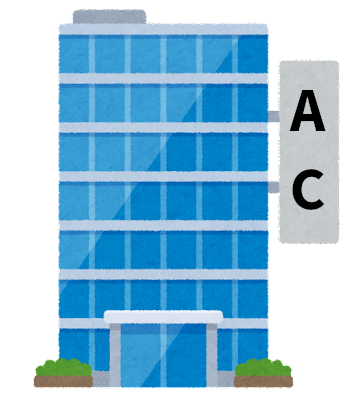
\includegraphics[width=0.15\textwidth]{images/ac_games.png}};
    \node[below=0cm of acgames] (acgames-name) {AC-Games};
    
    \node[left=3cm of acgames] (nutzer) {
\includegraphics[width=0.15\textwidth]{images/game_friends.png}};
    \node[below=0cm of nutzer] (nutzer-name) {Nutzer:innen};
    
    
    \draw<1-3>[-stealth] (walter) -- node[below] (ceo) {CEO}  (acgames);
    \draw<1>[-stealth] (nutzer) -- node[below] (geld) {Geld} (acgames);
    
    % Finanzkrise 2
    
    \draw<2->[-stealth, red] (nutzer) -- node[below] (geld) {Geld} (acgames);
    
    \node<2->[above=1cm of geld] (finanzkrise) {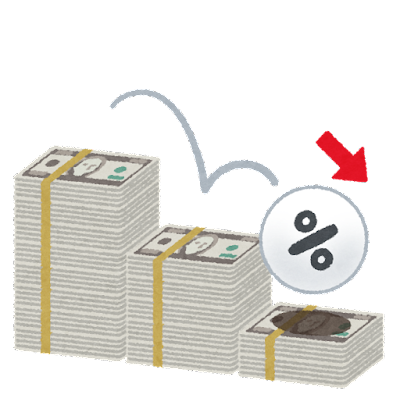
\includegraphics[width=0.12\textwidth]{images/money_down.png}};
    \node<2->[below=0cm of finanzkrise] (finanzkrise-name) {Finanzkrise};
    \draw<2->[dotted, red] (finanzkrise-name) -- (geld);
    
    % App Stores machen obsolet 3
    
    \node<3->[below=0.5cm of geld] (apps) {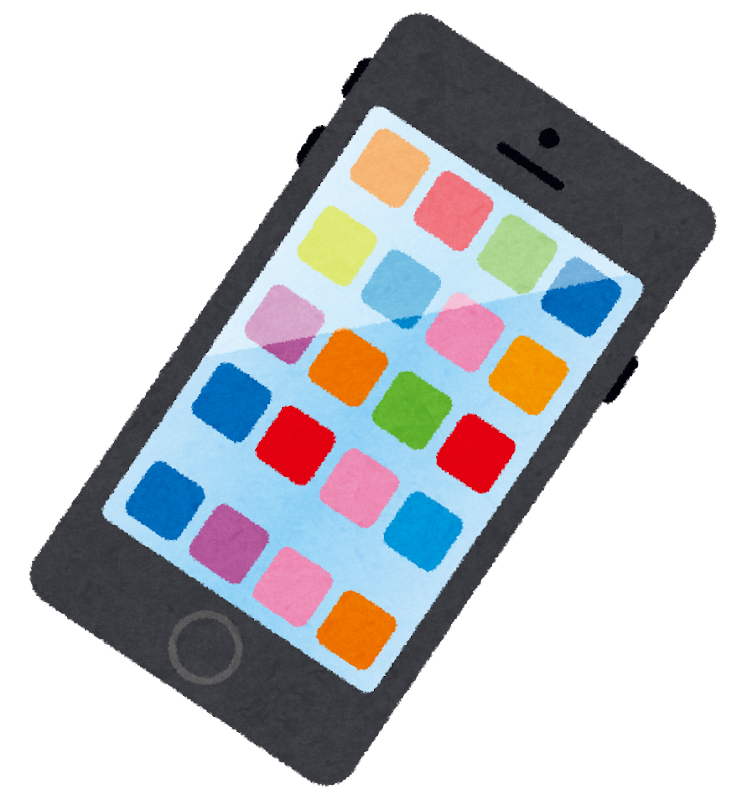
\includegraphics[width=0.10\textwidth]{images/smartphone.png}};
    \node<3->[below=0cm of apps] (apps-name) {App-Stores};
    \draw<3->[dotted, red] (apps) -- (geld);
    
    % Bankrott
    
    \node<4->[left=2.7cm of walter] (batsu) {
\includegraphics[width=0.2\textwidth]{images/batsu.png}};
    \draw<4->[-stealth, red] ([yshift=1mm]acgames.east) -- node[above] {Droht Bankrott} ([yshift=1mm]walter.west);
    \draw<4->[-stealth] ([yshift=-1mm]walter.west) -- node[below] (ceo) {CEO} ([yshift=-1mm]acgames.east);
  \end{tikzpicture} 
\end{frame}
\begin{frame}{Ein Angebot}
  \centering
  
  \note<1->[item]{Nachgrübeln was zu tun}
  \note<1->[item]{Plötzlich ein Angebot}
  \note<2->[item]{Firma "Data Broker GmbH" will Firma übernehmen \begin{itemize}
      \item Bietet Geld. (KLICK) VIEL Geld
  \end{itemize}}
  \note<4->[item]{Mitarbeiter fragen sich: Woher der hohe Preis?}
  \note<4->[item]{Gesammelte Daten sind nur für Transaktionen Wichtige}
  
  \begin{tikzpicture}
    \node<1-3> (walter) {
\includegraphics[width=0.15\textwidth]{images/walter.png}};
    \node<1-3>[below=0mm of walter] (walter-name) {Walter};
    
    \node<2-3>[right=4cm of walter] (databroker) {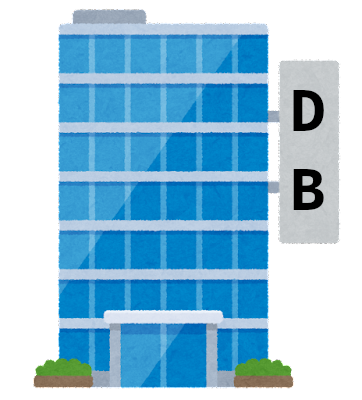
\includegraphics[width=0.15\textwidth]{images/data_broker.png}};
    \node<2-3>[below=0cm of databroker] (databroker-name) {Data Broker GmbH};
    
    % Data Broker kommt
    
    \draw<2-3>[stealth-] ([yshift=1mm]databroker.west) -- node[above] (acgames-name) {AC-Games}  ([yshift=1mm]walter.east);
    \node<2-3>[above=0cm of acgames-name] (acgames) {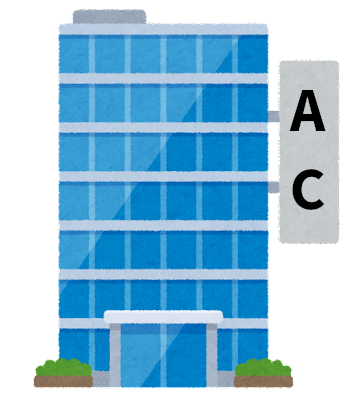
\includegraphics[width=0.075\textwidth]{images/ac_games.png}};
    \draw<2>[stealth-] ([yshift=-1mm]walter.east) -- node[below] {
\includegraphics[width=0.075\textwidth]{images/dollar_bill.png}}  ([yshift=-1mm]databroker.west);
    
    % MORE MONEY
    
    \draw<3>[stealth-] ([yshift=-1mm]walter.east) -- node[below] {
\includegraphics[width=0.1\textwidth]{images/money_bag_dollar.png}} ([yshift=-1mm]databroker.west);
    
    % Warum so viel geld?
    
    \node<4-> (typ) {
\includegraphics[width=0.45\textwidth]{images/pose_shinpai_fukidashi_man.png}};
    \node<4->[above=0cm of typ.center] (money) {
\includegraphics[width=0.18\textwidth]{images/money_bag_dollar.png}};
    
  \end{tikzpicture} 
\end{frame}

\begin{frame}{Ein Angebot}
  \centering
  
  \note[item] {Pro \begin{itemize}
      \item Firma bleibt relativ sicher bestehen
      \item Spieler und ihr Investment werden nicht im Stich gelassen
  \end{itemize}}
  \note[item]{Contra \begin{itemize}
      \item Daten in der Hand von Datenhändler \begin{itemize}
          \item Hoher Preis wird wohl seinen Grund haben
          \item Wahrscheinlich nicht aus reiner Wohltat
      \end{itemize}
  \end{itemize}}
  \note[item]{Alternativen \begin{itemize}
      \item Crowdfunding
      \item Vielleicht an dieser Stelle zu spät, aber hätte sich ein anderes Produkt überlegen können \begin{itemize}
          \item Haben ja schon Jahre vorher gemerkt, dass es mit ihrem Produkt abwärtsgeht
      \end{itemize}
  \end{itemize}}
  
  \Large
  Sollte Walter AC-Games an Data Broker verkaufen?\\
  Wenn nein, gibt es eine Alternative?
  
  
\includegraphics[width=0.425\textwidth]{images/discussion.png}
\end{frame}

\begin{frame}{Ein Angebot}
  \centering
  
  \note[item] {Pro \begin{itemize}
    \item Offensichtlich: Firma soll überleben
  \end{itemize}}
  \note[item]{Contra \begin{itemize}
    \item Finanzkrise ist ja nicht einziger Grund
    \item App Stores etc. bieten scheinbar besseren Service
    \item In-Game Käufe lassen nach $\Rightarrow$ hört sich eher nach Problem mit Produkt selbst an
  \end{itemize}}
  
  \Large
  Wie bewertet ihr, dass AC-Games trotz finanzieller Schwierigkeiten ihr Portal weiter betreiben wollen? 
  
  
\includegraphics[width=0.425\textwidth]{images/discussion.png}
\end{frame}


\begin{frame}{Übernahme}
    
\end{frame}

\begin{frame}{Die Ultimative Slot Machine}
	\centering

	\note[item] {Gehen zum Anfang der Firma zurück}
	\note[item] {Am Anfang der Firma war Datenschutz keine hohe Priorität}
	\note[item] {Alter Blog-Eintrag von Walter:}

	\note<2->[item] {Beschreibt die "Ultimative Slot Machine" \begin{itemize}
			\item Beschreibt Glücksspielmaschine, die sich dem Spieler anpasst
			\item Dazu müssten Verhaltensdaten gesammelt werden
		\end{itemize}
	}
	\note<2->[item] {Gab noch andere Ideen was mit den Daten möglich ist (nur intern) \begin{itemize}
			\item Spieler künstlichem Stress aussetzen $\Rightarrow$ Wahl-/Kaufverhalten beeinflussen \begin{itemize}
				      \item Unvorteilhafte Entscheidungen treffen
			      \end{itemize}
		\end{itemize}
	}
	\note<3->[item] {
		Ideen wurden verworfen \begin{itemize}
			\item Datenschutz wurde Walter wichtiger
			\item Rechtlich nicht so einfach
		\end{itemize}
	}

	\begin{tikzpicture}
		\node<2-3> (slotmachine) {
\includegraphics[width=0.50\textwidth]{images/gambling.png}};
		\node<3> (batsu) {
\includegraphics[width=0.50\textwidth]{images/batsu.png}};
	\end{tikzpicture}
\end{frame}

\begin{frame}{Die Ultimative Slot Machine}
	\centering
	\note[item]{Wäre alles Theorie $\Rightarrow$ alles gut}
	\note<2>[item]{Stellt sich heraus: Diese Daten tatsächlich gesammelt}
	\note<2>[item]{Systeme hätten umprogrammiert werden müssen}
	\note<3>[item]{Kathleen: Überblick über Speicherung der Daten \begin{itemize}
			\item Aber keine Ressoucen das zu beheben.
		\end{itemize}}
	\note<3>[item]{$\Rightarrow$ Speicherung der Daten setzte sich fort.}

	\begin{tikzpicture}
		\node<2-> (server) {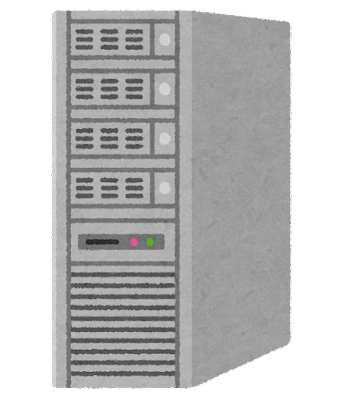
\includegraphics[height=0.2\textwidth]{images/server.png}};
		\node<2->[below = 0cm of server] (server-name) {Daten};
		\node<3>[left = 3cm of server] (kathleen) {
\includegraphics[height=0.2\textwidth]{images/kathleen.png}};
		\node<3>[below = 0cm of kathleen] (kathleen-name) {Kathleen};

		\draw<3>[-stealth] (kathleen) -- (server);
	\end{tikzpicture}
\end{frame}

\begin{frame}{Die Ultimative Slot Machine}
	\centering

	\note[item]{Datenschutzaudit macht auch darauf aufmerksam \begin{itemize}
			\item auch wenn es (scheinbar) nach AGBs rechtens ist
			\item Aber DSGVO: gesammelte Daten müssen bestimmten Zweck gewidmet sein. Sonst Sammlung unrechtens
		\end{itemize}}
	\note[item]{hat Data Broker auf AC-Games aufmerksam wurde \begin{itemize}
			\item hat Interesse an den Verhaltensdaten der Nutzer
		\end{itemize}
	}
	\note[item]{ Nicht mal AGB müssgen geändert werden \begin{itemize}
			\item "Idealfall": Die Nutzer bekommen gar nichts mit
		\end{itemize}
	}

	\begin{tikzpicture}
		\node (inspector) {
\includegraphics[width=0.25\textwidth]{images/inspector.png}};
		\node<2->[above right=1.5cm and 1cm of inspector.center] (speech) {\includesvg[width=0.25\textwidth]{images/Speech_bubble}};
		\node<2->[above right=-0.6cm and 0cm of speech.center, label={[align=center]Schon bisschen\\komisch...}] (komisch) {};

	\end{tikzpicture}
\end{frame}

\begin{frame}{Die Ultimative Slot Machine}
	\centering

	\note[item] {Pro \begin{itemize}
			\item Sollte das komisch finden, dass Daten so lange gespeichert werden.
			\item Ist die Einzige die einen Überblick über Datenerfassung hat
		\end{itemize}}
	\note[item]{Contra \begin{itemize}
			\item Hatte nicht genug Ressourcen \begin{itemize}
				      \item Vielleicht zu sehr mit anderen Dingen beschäftigt.
				      \item Walter hätte eingreifen können. Sollte sich ein Bild davon machen.
			      \end{itemize}
		\end{itemize}}

	\Large
	Welche Verantwortung hatte Kathleen, die Datenerfassung zu hinterfragen, nachdem die Daten so lange nicht benutzt wurden?

	
\includegraphics[width=0.425\textwidth]{images/discussion.png}
\end{frame}

% https://www.irasutoya.com/2019/04/blog-post_87.html
\begin{frame}{Hank}
	\centering

	\note<1->[item]{Hank neuer Mitarbeiter bei AC-Games}

	\note<2->[item]{Ist Datenbankadmin}
	\note<2->[item]{Hat nicht vor lange bei der Firma zu bleiben}
	\note<2->[item]{Hat Walters alten Blogpost gelesen}

	\note<3->[item]{Ist auch verwundert über hohen Preis}
	\note<3->[item]{Will schauen was aus den Daten rauszuholen ist}


	\begin{tikzpicture}
		\node<1-2> (hank) {
\includegraphics[height=0.15\textwidth]{images/hank}};
		\node[below =0cm of hank] (hank-name) {Hank};

		% Pack Server hin

		\node<2->[right =4cm of hank] (server) {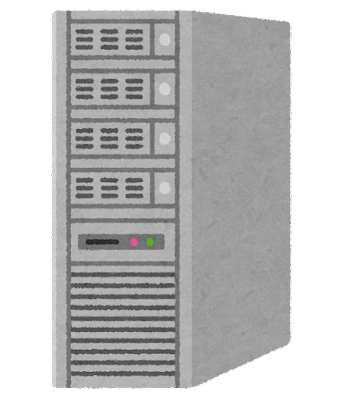
\includegraphics[height=0.15\textwidth]{images/server}};
		\node<2->[below =0cm of server] (server-name) {Datenbank};

		\draw<2->[-stealth] (hank) -- node[above] {Admin} (server);

		% "Mal rumprobieren"
		\node<3-> (hank) {
\includegraphics[height=0.15\textwidth]{images/hank_hmm}};
		\node<3->[above right=-8mm and 0mm of hank] (speech) {\includesvg[width=0.25\textwidth]{images/thought_bubble}};
		\node<3->[above right = -3mm and -1mm of speech.center, label={[align=center]Mal schauen}] (wenig-daten) {};
	\end{tikzpicture}
\end{frame}

\begin{frame}{Das Experiment}
	\centering

	\note<1-4>[item]{Berechnungen auf dem Daten}
	\note<2-4>[item]{Nutzer lassen sich nach Verhalten in Kategorien einteilen}
	\note<3-4>[item]{Stress-Typen}
	\note<4>[item]{Neugier-Typen}
	\note<4>[item]{Nicht wirklich beschrieben, was diese ausmacht \begin{itemize}
			\item Auch nicht so wichtig
		\end{itemize}}
	\note<5->{Im In-Game Shop \begin{itemize}
			\item Programmiert künstlichen Zähler (\#Vorrätige Exemplare)
			\item Auf Nutzer-Typ angepasst
			\item Für Stress-Typen \begin{itemize}
				      \item Anfangs 2-stellige Zahl
				      \item Tickt langsam runter
			      \end{itemize}
			\item Für Neugier-Typen \begin{itemize}
				      \item Zeigt zuerst keine Zahl sondern \enquote{Vorrat prüfen} Knopf
				      \item Dann wird \enquote{Nur noch 1 Exemplar} angezeigt
			      \end{itemize}
		\end{itemize}}

	\visible<2->{\begin{tabular}{c|lll}
			\textbf{Typ} & \textbf{Nutzer:innen}                                  \\\hline \hline\onslide<3->
			Stress       & Bob L.                & Lina M.  & \dots  \onslide<4-> \\\hline
			Neugier      & Katie A.              & Chris O. & \dots               \\
			\vdots       & \dots                 &          &
		\end{tabular}}
\end{frame}

\begin{frame}{Die Ergebnisse}
	\centering

	\note<1->{Nächster Abend: Hank prüft die Verkaufszahlen}
	\note<2->{Umgestaltung des Shop hat Kaufverhalten stark beeinflusst}
	\note<3->{Fragt sich: Was kann noch alles mit den Daten angestellt werden. \begin{itemize}
			\item mit Kunden von AC-Games
			\item vielleicht auch außerhalb?
		\end{itemize}}

	\begin{tikzpicture}
		\node<1> (hank) {
\includegraphics[width=0.15\textwidth]{images/hank}};
		\node[below =0cm of hank] (hank-name) {Hank};

		\node<2> (hank) {
\includegraphics[width=0.15\textwidth]{images/hank_surprise}};
		\node<2>[right =2cm of hank] (more_money) {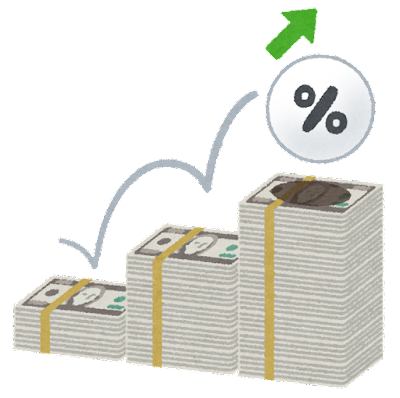
\includegraphics[width=0.2\textwidth]{images/more_money}};

		\node<3> (hank) {
\includegraphics[width=0.15\textwidth]{images/hank_worried}};
		\node<3->[above right=-8mm and -2mm of hank] (speech) {\includesvg[width=0.25\textwidth]{images/thought_bubble}};
		\node<3->[above right = -5mm and -1mm of speech.center, label={[align=center]Damit kann man\\echt Mist bauen...}] (wenig-daten) {};
	\end{tikzpicture}
\end{frame}


\begin{frame}{Suche nach einer Lösung}
	\centering

	\note[item] {Sollte Hank sich hier an die Auflagen halten?}
	\note[item] {Möglichkeiten: \begin{itemize}
			\item Walter etc. Bescheid sagen
			\item Datenbank trotzdem bearbeiten und anonymisieren
		\end{itemize}}

	\Large
	Was würdet ihr Hank raten?

	
\includegraphics[width=0.425\textwidth]{images/discussion.png}
\end{frame}

\begin{frame}{Suche nach einer Lösung}
	\centering

	\note[item]<1->{Entscheidung: Bearbeitung der Datenbank}
	\note[item]<1->{Daten so aussehen lassen, als wären sie immer so erhoben worden.}
	\note[item]<1->{Pseudonymisiert Kunden-IDs}

	\note[item]<2->{Speichert Zuordnungstabelle auf privatem USB Stick}

	\begin{tikzpicture}

		\node (hank) {
\includegraphics[width=0.15\textwidth]{images/hank_pc}};
		\node[below=0cm of hank] (hank-name) {Hank};
		\node<2>[above right=-8mm and -2mm of hank] (speech) {\includesvg[width=0.3\textwidth]{images/thought_bubble}};
		\node<2>[above right=-5mm and -1mm of speech.center, label={[align=center]Ich anonymisiere\\die Datenbank.}] (eingreifen) {};

    \node<3->[right = 4cm of hank] (usb) {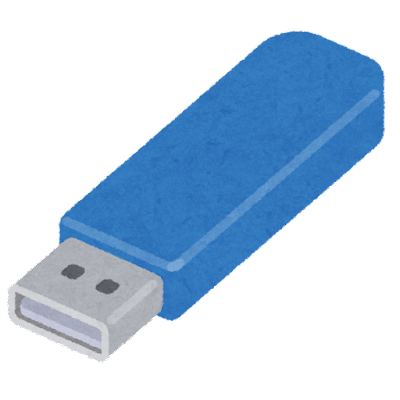
\includegraphics[width=0.15\textwidth]{images/usb_memory_stick}};

    \draw<3->[-stealth] (hank) -- node[above] {Zuordnungstabelle} (usb);

	\end{tikzpicture}

\end{frame}

\begin{frame}{Suche nach einer Lösung}
	\centering

	\note[item] {Pro: \begin{itemize}
        \item Theoretisch Pseudonymisierung
		\end{itemize}}
	\note[item] {Contra: \begin{itemize}
        \item Zuordnungstabelle offensichtlich komisch
        \item War nicht der Audit schon? Weiß Data Broker nicht genau, welche Daten erhoben wurden? \begin{itemize}
            \item Das würden die doch merken
        \end{itemize}
		\end{itemize}}

	\Large
    Haltet ihr es für vertretbar, dass Hank trotz Anweisungen die Datenbank bearbeitet hat?

	
\includegraphics[width=0.425\textwidth]{images/discussion.png}
\end{frame}

\section{International Data Privacy Principles \cite{zankl_international_2014}}

\begin{frame}{International Data Privacy Principles}

    % Einleitung
    \note<1>[item]{13 Ethische Prinzipien für Umgang mit Daten für Firmen}
    \note<1>[item]{Erarbeitet von Wolfang Zankl - Institut für Zivilrecht Wien}
    \note<1>[item]{Orientieren sich an den Datenschutzstandards von Ländern weltweit}
    \note<1>[item]{Viele davon relativ selbsterklärend.}
    \note<1>[item]{Meine Übersetzung}


    % Prinzip anzeigen
    \visible<2->{Eine Firma, die persönliche Daten nutzt, soll\dots}

    \only<2->{\begin{block}{Prinzip 1 \cite{zankl_international_2014}}
        \dots die jeweiligen nationalen and internationalen Regelungen einhalten die Datenschutz als Gegenstand haben. 
    \end{block}}

    % Genauer Verwendungszweck
    \note<3>[item]{Art. 5 Abs 1b: Genauer Verwendungszweck \begin{itemize}
        \item Kennen zwar ihre AGB nicht, aber
        \item Für die meisten Daten $\exists$ kein Verwendungszweck
        \item $\Rightarrow$ Es kann auch keiner angegeben worden sein.
    \end{itemize}}

    \only<3->{
        \textcolor{red}{Nein} 
    }
    \only<3>{Art. 5 Abs. 1b DSGVO: Genauer Verwendungszweck muss exakt und eindeutig festgehalten werden. }
    
    % Sammlung von Daten außerhalb von designiertem Zweck nicht erlaubt 
    \note<4>[item]{Nicht nur Walter etc. verstoßen dagegen sondern auch Hank \begin{itemize}
        \item Sein Experiment: Unauthorisierte Nutzung
    \end{itemize}}

    \only<4>{Art. 5 Abs. 1c DSGVO: Jegliche Sammlung und Nutzung außerhalb dessen ist nicht zulässig.}
    
    % Löschung erhobener Daten
    \note<5>[item]{Wer immer Verantwortung für Datenspeicherung hat (Walter, Kathleen, etc.), hat es nicht getan}

    \only<5>{Art. 5 Abs. 1e DSGVO: Erhobene Daten müssen gelöscht werden, sollten sie nicht mehr gebraucht werden.}

\end{frame}

\begin{frame}{International Data Privacy Principles}

    \note<1->[item]{
        Hank hat definitiv gebrochen. \begin{itemize}
            \item Laden der Zuordnungstabelle auf einen privaten USB Stick: 
        \end{itemize}
    }

    Eine Firma, die persönliche Daten nutzt, soll\dots

    \begin{block}{Prinzip 2 \cite{zankl_international_2014}}
        \dots durch Einhalten aktueller Sicherheitsstandards, unbefugten Zugriff und Verarbeitung, sowie Löschung und Verlust zu verhindern.
    \end{block}
    \only<2>{
        AC-Games: \textcolor{gold}{Vielleicht} Wissen nicht viel über die \emph{Sicherung} der Daten.
    }
    \only<3->{
        Hank: \textcolor{red}{Nein} Er hat die Zuordnungstabelle auf einen USB Stick geladen. Das kann einfach zu Verlust führen.
        }

\end{frame}

\begin{frame}{International Data Privacy Principles}

    \note<1->[item]{
        Hank hat definitiv gebrochen. \begin{itemize}
            \item Eigenes Herumhantieren mit den Daten
        \end{itemize}
    }

    Eine Firma, die persönliche Daten nutzt, soll\dots

    \begin{block}{Prinzip 3 \cite{zankl_international_2014}}
        \dots eine für Kunden einfach verständliche Datenschutzrichtlinie aufstellen und den Kunden erlauben die verantwortliche Person persönlich zu kontaktieren. Darüber hinaus muss die Richtline beschreiben welche Daten zu welchem Zweck erhoben werden [und] wie die Daten genutzt werden [\dots].
    \end{block}
    \only<2->{
        \textcolor{red}{Nein} Bereits gesagt: Es gab keinen Zweck für viele der Daten, deswegen kann auch niemand etwas über den Zweck sagen.
    }

\end{frame}

\begin{frame}{International Data Privacy Principles}

    \note<1->[item]{Könnte man sagen, aber trotzdem dubios}
    \note<2->[item]{Frage: Darf man sowas mit AGB überhaupt machen?}

    Eine Firma, die persönliche Daten nutzt, soll\dots

    \begin{block}{Prinzip 5 \cite{zankl_international_2014}}
        \dots Daten nicht an unauthorisierte Dritte weiter geben, außer [\dots] der Kunde hat zugestimmt. [\dots] 
    \end{block}

    \only<2->{
        \textcolor{green}{Ja?} Scheinbar müssen bei der Übernahme die AGB nicht geändert werden. Also müsste die Übernahme unter den vorherigen AGB rechtens sein. 
    }

\end{frame}

\begin{frame}{International Data Privacy Principles}

    \note<1->[item]{Einfache Sache}

    Eine Firma, die persönliche Daten nutzt, soll\dots

    \begin{block}{Prinzip 6 \cite{zankl_international_2014}}
        \dots nur nötige Daten sammeln.
    \end{block}

    \only<2->{
        \textcolor{red}{Nein} Offensichtlich
    }

\end{frame}

\begin{frame}{International Data Privacy Principles}

    Eine Firma, die persönliche Daten nutzt, soll\dots

    \begin{block}{Prinzip 7 \cite{zankl_international_2014}}
        \dots die gesammelten Daten auf faire Art und Weise benutzen [\dots] und nur zum Zweck der für die Firma nötigen Zwecke.
    \end{block}

    \only<2>{
        AC-Games: \textcolor{green}{Ja} Sie haben zwar zu viele Daten gesammelt, aber wirklich nur Daten benutzt, die sie brauchen.
    }
    \only<3->{
        Hank: \textcolor{red}{Nein} Er hat unauthorisiert gesammelte Daten zu unauthorisierten Zwecken benutzt um die Nutzer zu ihren Ungunsten zu beeinflussen.
    }

\end{frame}

\begin{frame}{International Data Privacy Principles}

    Eine Firma, die persönliche Daten nutzt, soll\dots

    \begin{block}{Prinzip 8 \cite{zankl_international_2014}}
        \dots keine Daten an Instanzen weitergeben, die internationale Datenschutzstandards nicht einhalten. 
    \end{block}

    \only<2->{
        \textcolor{orange}{Dubios} Wir wissen nicht \emph{genau}, dass Data Broker schlecht mit den Daten umgeht, aber es ist doch sehr naheliegend.
    }

\end{frame}

\begin{frame}{International Data Privacy Principles}

    Eine Firma, die persönliche Daten nutzt, soll\dots

    \begin{block}{Prinzip 10 \cite{zankl_international_2014}}
        \dots Daten nur so lang wie nötig aufbewahren.
    \end{block}

    \only<2->{
        \textcolor{red}{Nein} Die Daten waren nie nötig, also ist der erlaubte Speicherzeitraum genau null Sekunden. 
    }

\end{frame}


\begin{frame}{Fazit}

	\note<1->[item]{
		Erfüllt viele ethische Prinzipien nicht
	}
	\note<2->[item]{
		Also unethisch mit den Daten umgegangen \begin{itemize}
			\item Viele unnötige Daten gesammelt
			\item Hank: Hat manche Daten in gefahr gebracht
		\end{itemize}
	}
	\note<3->[item]{
		Dazu: DSGVO nicht erfüllt \begin{itemize}
			\item Unnötige Daten gesammelt
			\item Über benötigten Zeitraum hinaus gespeichert
		\end{itemize}
	}
	\note<4->[item]{Sowohl ethische Prinzipien und Gesetz gebrochen \begin{itemize}
			\item Erinnerung Anfang: Ethik und Gesetz sind verbunden
		\end{itemize}}

	\begin{itemize}
		\item<1-> AC-Games erfüllt viele der Prinzipien nicht \begin{itemize}
			\item<2-> Anhand der Prinzipien nicht ethisch mit den Daten umgegangen
		\end{itemize}
		\item<3-> Auch DSGVO ist nicht erfüllt
		\item<4-> Sowohl ethische Prinzipien und Gesetz gebrochen
	\end{itemize}
\end{frame}


\nocite{mifune}

\begin{frame}{Literatur}
\printbibliography[heading=none]
\end{frame}


\end{document}
